% Subespacios, producto cuña y determinante
% Números y figuras PNG: apunte/scripts/cap06_cuna_determinante.py (uv run python apunte/scripts/cap06_cuna_determinante.py)
\chapter{Subespacios, producto cuña y determinante}\label{cap:subespacios}\label{sec:bloque-algebraico}

\section{La idea}

Este capítulo responde preguntas que en el campo aparecen todo el tiempo: ¿están alineados
estos tres mojones?, ¿dónde se cortan dos alineaciones?, ¿cuánta superficie encierra esta
poligonal?, ¿cuánto agranda las áreas esta transformación? Todas se contestan con una misma
herramienta, el \emph{producto cuña}, que mide áreas \emph{con signo}. El determinante es su
versión para \(n\) vectores de \(\R^n\), y el núcleo de una matriz es lo que queda cuando ese
número se anula.

\paragraph{Convenciones del capítulo.} Puntos y vectores en minúscula cursiva (\(p\), \(u\),
\(v\)), escritos en el texto como \((u_x,u_y)\) o \((u_1,u_2,u_3)\) y en las cuentas como
columnas; matrices en mayúscula itálica (\(A\), \(M\)). En coordenadas homogéneas del plano
(capítulo~\ref{cap:afines}) el punto \((x,y)\) se escribe \((x,y,1)\) y la recta
\(ax+by+c=0\), \((a,b,c)\); \(\times\) es el producto vectorial de \(\R^3\) y \(\wedge\) el
producto cuña.

Primero el mapa: cada operación del álgebra se lee como una pregunta geométrica. Lo armamos así y dejamos las cuentas para la sección siguiente.

\subsection{Del álgebra a la geometría: qué pregunta cada operación}\label{sec:algebra-geometria}

\textbf{Desarrollo.} El hilo de la materia es siempre el mismo: una operación algebraica,
en apariencia abstracta, resulta ser exactamente la pregunta geométrica que necesitábamos.
Conviene tener el mapa antes de las cuentas.

\begin{center}
\begin{tabularx}{\textwidth}{>{\bfseries}p{34mm} X X}
\toprule
Operación & Qué calcula & Qué pregunta geométrica responde\\
\midrule
Producto interno \(u\cdot v\) & un número & ¿son ortogonales? ¿cuánto se proyecta uno
sobre otro? En homogéneas: ¿el punto está en la recta?\\
Producto vectorial \(u\times v\) & un vector normal a ambos & ¿cuál es la recta que une dos
puntos? ¿cuál es el punto donde se cortan dos rectas? ¿qué área orientada forman?\\
Determinante \(\det[u\ v\ w]\) & un número & ¿están alineados tres puntos? ¿son
linealmente dependientes tres vectores? ¿qué volumen orientado forman?\\
Producto exterior \(u\wedge v\) & un bivector (área orientada) & lo mismo que el
vectorial, pero en cualquier dimensión\\
Núcleo de \(A\) & un subespacio & ¿qué vectores aplasta \(A\) a cero? Si hay alguno,
\(\det A=0\)\\
Autovectores de \(A\) & vectores con \(Av=\lambda v\) & ¿qué direcciones deja quietas
\(A\)? En homogéneas: ¿qué puntos deja fijos la transformación?\\
\bottomrule
\end{tabularx}
\end{center}

\begin{idea}[La cadena]
incidencia \(\to\) unión de puntos \(\to\) alineación \(\to\) determinante \(\to\)
núcleo \(\to\) autovectores \(\to\) puntos fijos. Cada eslabón se deduce del anterior;
es lo que desarrollan las secciones siguientes de este capítulo.
\end{idea}

\begin{idea}[El producto cuña como detector de colinealidad]
El producto cuña, detector de colinealidad, sirve primero para construir un polinomio cuyas
raíces son los autovalores, y luego para hallar los autovectores como el subespacio nulo
de unas matrices que armamos.
\end{idea}

\subsection{Subespacios lineales y afines}\label{sec:subespacios-lineales-afines}

Una recta del plano puede pasar por el origen o no. La diferencia parece menor, pero decide
qué operaciones se le pueden aplicar: la suma de dos vectores de la recta \(y=2x\) sigue en
esa recta, y la de dos puntos de \(y=2x+1\) no.

\begin{definicion}[Subespacio lineal y subespacio afín]\label{def:subespacio}
Un \emph{subespacio lineal} de \(\R^n\) es un conjunto \(S\) no vacío cerrado por sumas y por
múltiplos: si \(u,v\in S\) y \(t\in\R\), entonces \(u+v\in S\) y \(tu\in S\). En particular
\(0\in S\): todo subespacio lineal pasa por el origen. Un \emph{subespacio afín} es un
subespacio lineal trasladado, \(p_0+S=\{p_0+s:\ s\in S\}\); pasa por el origen sólo si
\(p_0\in S\), y en ese caso es lineal. La \emph{dimensión} de \(p_0+S\) es la de \(S\).
\end{definicion}

Cada subespacio se describe de dos maneras, que conviene saber pasar de una a la otra:
\begin{itemize}
  \item \textbf{Paramétrica} (cómo se recorre): \(x=p_0+t\,d\) para una recta,
  \(x=p_0+s\,u+t\,v\) para un plano; los vectores \(d\), o \(u,v\), generan \(S\).
  \item \textbf{Implícita} (qué ecuaciones cumple): \(ax+by=c\) para una recta del plano,
  \(n\cdot x=c\) para un plano de \(\R^3\). Es lineal si \(c=0\) y afín si \(c\neq0\).
\end{itemize}
Por ejemplo, la recta que pasa por \(p_0=(0,1)\) con dirección \(d=(1,2)\) es
\((x,y)=(0,1)+t(1,2)\) en forma paramétrica; eliminando \(t\) queda \(2x-y=-1\), una recta
afín, paralela a la recta lineal \(2x-y=0\). Pasar de la paramétrica a la implícita es buscar
un vector \emph{perpendicular a los generadores}; ahí entra el producto cuña
(ejercicio~\ref{ex:cuna-plano-afin}).

\begin{idea}[Afín es lineal corrido: misma dirección, otro lugar]
Un subespacio afín tiene la misma ``forma'' que su subespacio lineal paralelo; sólo está
desplazado. Las ecuaciones homogéneas (\(=0\)) describen subespacios lineales; un término
independiente no nulo los traslada. En coordenadas homogéneas del capítulo~\ref{cap:afines}
esta diferencia desaparece: una recta afín del plano es un plano lineal de \(\R^3\) que pasa
por el origen.
\end{idea}

\subsection{El producto cuña en el plano: área con signo}\label{sec:cuna-plano}

Dos vectores \(u\), \(v\) del plano, puestos con su origen común, forman un paralelogramo.
Su área es un número positivo; pero si además registramos en qué sentido hay que girar para
ir de \(u\) a \(v\), obtenemos un número con signo, y ese número es mucho más útil.

\begin{definicion}[Producto cuña de dos vectores del plano]\label{def:cuna-plano}
Para \(u=(u_x,u_y)\) y \(v=(v_x,v_y)\),
\[
  u\wedge v=u_xv_y-u_yv_x=\det\begin{pmatrix}u_x&v_x\\u_y&v_y\end{pmatrix}.
\]
Su valor absoluto es el área del paralelogramo de lados \(u\) y \(v\); es positivo si el giro
más corto de \(u\) hacia \(v\) es antihorario y negativo si es horario.
\end{definicion}

\begin{figure}[htbp]
\centering
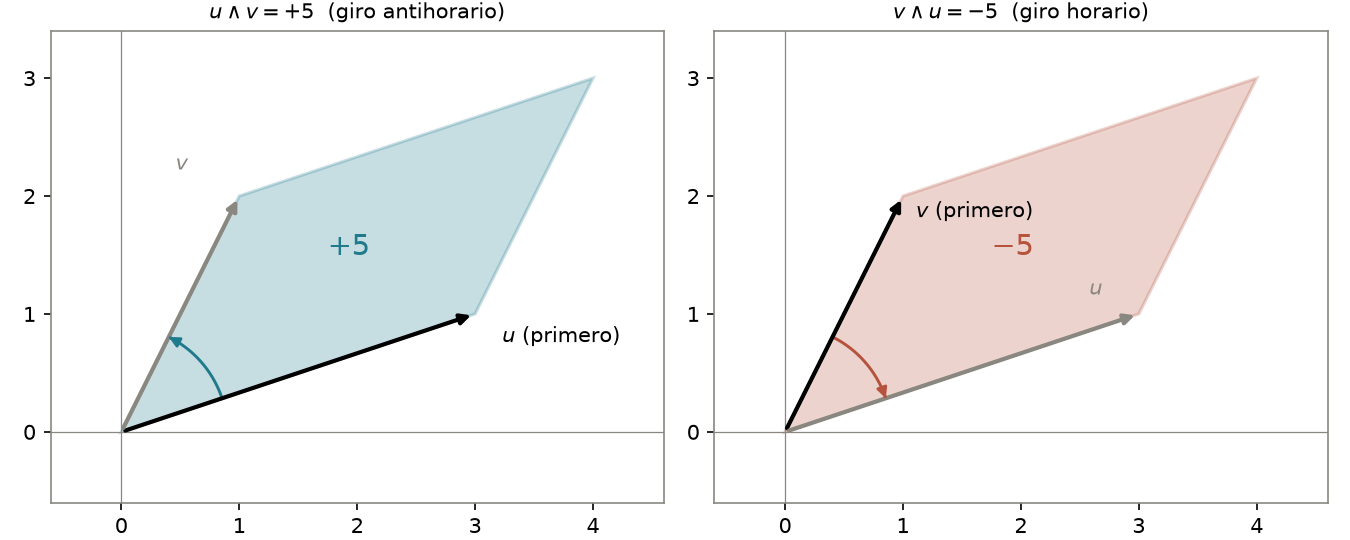
\includegraphics[width=.92\linewidth]{figuras/cuna-determinante/cuna_paralelogramo.png}
\caption{El mismo paralelogramo, de lados \(u=(3,1)\) y \(v=(1,2)\), con los dos órdenes.
Izquierda: de \(u\) a \(v\) se gira en sentido antihorario y \(u\wedge v=+5\). Derecha: de
\(v\) a \(u\) se gira en sentido horario y \(v\wedge u=-5\). Generada con
\texttt{apunte/scripts/cap06\_cuna\_determinante.py}.}
\label{fig:cuna-paralelogramo}
\end{figure}

La fórmula se lee en la figura~\ref{fig:cuna-paralelogramo}: el rectángulo que encierra el
paralelogramo de \(u=(3,1)\) y \(v=(1,2)\) mide \(4\times3=12\); le sacamos dos triángulos de
área \(\tfrac32\), dos de área \(1\) y dos rectangulitos de área \(1\), y queda
\(12-3-2-2=5=3\cdot2-1\cdot1\). Tres propiedades lo caracterizan:
\begin{itemize}
  \item \textbf{lineal en cada vector}: duplicar un lado duplica el área;
  \item \textbf{antisimétrico}: \(v\wedge u=-\,u\wedge v\), cambiar el orden cambia el
  sentido;
  \item \(u\wedge u=0\): un vector consigo mismo no encierra área.
\end{itemize}

\begin{idea}[El signo del área es el sentido de giro]
El producto cuña no sólo mide cuánta superficie hay entre dos vectores: dice de qué lado del
primero está el segundo. Positivo, a la izquierda (giro antihorario); negativo, a la derecha;
cero, sobre la misma recta. Ese signo es el que, sumado vértice por vértice, da el área de
cualquier polígono (sección~\ref{sec:poligono-cunas}).
\end{idea}

\unidadInteractiva{07a_cuna_determinante}{Cuña y determinante: el detector de colinealidad}{Explorá: en el caso «v gira alrededor de u = (3, 1)» mové el ángulo de \(v\) y mirá cómo el área sube, se anula cuando \(v\) se alinea con \(u\) y cambia de signo al cruzar esa recta.}

\section{Construcciones, cuentas y ejemplos}


Hacemos la cuenta de cada operación con su figura: producto interno, producto vectorial, determinante, núcleo, autovalores y formas lineales. El orden es el de la cadena de la sección anterior.

El objetivo es que la parte geométrica y la parte algebraica se conecten, y entender por qué
el determinante tiene las propiedades ``mágicas'' que tiene. Lo que sigue reconstruye ese
razonamiento en orden.

\subsection{El cuña como detector de colinealidad}\label{sec:cuna-colinealidad}

\begin{proposicion}[El cuña se anula exactamente en los vectores dependientes]\label{prop:cuna-dependencia}
Para \(u,v\in\R^2\), \(u\wedge v=0\) si y sólo si \(u\) y \(v\) son linealmente dependientes,
es decir, si uno es múltiplo del otro (están sobre una misma recta por el origen).
\end{proposicion}

\begin{demostracion}
Si \(v=tu\), entonces \(u\wedge v=t\,(u\wedge u)=0\) por linealidad; lo mismo si \(u=tv\).
Recíprocamente, supongamos \(u\wedge v=u_xv_y-u_yv_x=0\). Si \(u=0\), son dependientes. Si
\(u\neq0\), el vector \(u^\perp=(-u_y,u_x)\) es no nulo y perpendicular a \(u\), y
\(u^\perp\cdot v=u_xv_y-u_yv_x=0\): \(v\) es perpendicular a \(u^\perp\), así que está en la
recta de dirección \(u\), y \(v=tu\) para algún \(t\).
\end{demostracion}

La demostración deja una lectura que vamos a usar todo el capítulo:
\(u\wedge v=u^\perp\cdot v\). El cuña es un producto interno con el vector \(u\) girado
\(90^\circ\); por eso mide cuánto se aparta \(v\) de la recta de \(u\). Tres puntos \(a,b,c\)
están alineados si y sólo si \((b-a)\wedge(c-a)=0\), y la mitad de ese número es el área con
signo del triángulo \(abc\).

\begin{ejemplo}[Área orientada de un paralelogramo y de un triángulo]\label{ej:cuna-area}
Para \(u=(3,1)\) y \(v=(1,2)\),
\[
  u\wedge v=3\cdot2-1\cdot1=5,\qquad v\wedge u=1\cdot1-2\cdot3=-5 :
\]
el paralelogramo mide \(5\) y de \(u\) a \(v\) se gira en sentido antihorario
(figura~\ref{fig:cuna-paralelogramo}). Para el triángulo de vértices \(a=(1,1)\),
\(b=(5,2)\), \(c=(2,4)\), restamos \(a\) para llevar un vértice al origen:
\[
  b-a=(4,1),\quad c-a=(1,3),\qquad
  \tfrac12\,(b-a)\wedge(c-a)=\tfrac12\,(4\cdot3-1\cdot1)=\tfrac{11}2=5{,}5 .
\]
El signo positivo dice que el recorrido \(a\to b\to c\) es antihorario; recorrido como
\(a\to c\to b\) da \(-5{,}5\). Los tres puntos no están alineados, porque el número no es
cero.
\end{ejemplo}

\paragraph{En el espacio: el cuña como vector normal.} Para \(u,v\in\R^3\) hay tres planos
coordenados y en cada uno el paralelogramo de \(u\) y \(v\) proyecta un área con signo. Esos
tres números,
\[
  u_2v_3-u_3v_2,\qquad u_3v_1-u_1v_3,\qquad u_1v_2-u_2v_1 ,
\]
son las componentes del producto vectorial \(u\times v\)
(sección~\ref{sec:vectorial}): un vector normal al plano de \(u\) y \(v\), de largo igual al
área del paralelogramo. Cada componente es un cuña de \(2\times2\) de las coordenadas que
quedan al tapar una. La lectura del producto vectorial como \emph{bivector}, un trozo de
plano orientado y no una flecha, es la de la sección~\ref{sec:exterior}. El análogo de la
proposición~\ref{prop:cuna-dependencia} sigue valiendo: \(u\times v=0\) si y sólo si \(u\) y
\(v\) son dependientes.

\subsection{El determinante como factor de área y de volumen}\label{sec:det-factor}

Una matriz \(M\) de \(2\times2\) lleva los vectores \(e_1=(1,0)\) y \(e_2=(0,1)\) a sus
columnas \(u\) y \(v\), y por lo tanto el cuadrado unidad al paralelogramo de \(u\) y \(v\),
de área con signo \(u\wedge v=\det M\). Como \(M\) es lineal, toda la grilla de cuadrados se
transforma en una grilla de paralelogramos iguales (figura~\ref{fig:cuna-grilla}); cualquier
región, aproximada por cuadraditos, cambia su área por el mismo factor.

\begin{figure}[htbp]
\centering
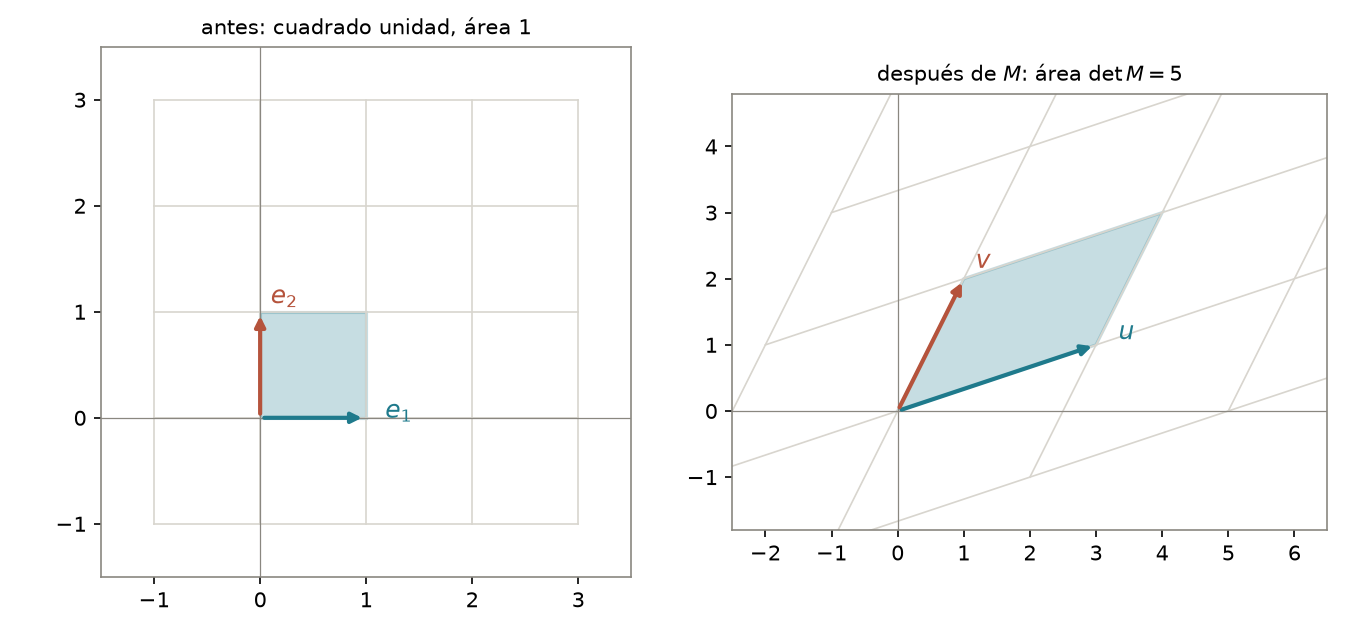
\includegraphics[width=.92\linewidth]{figuras/cuna-determinante/cuna_grilla.png}
\caption{La matriz \(M=\left(\begin{smallmatrix}3&1\\1&2\end{smallmatrix}\right)\), de
columnas \(u=(3,1)\) y \(v=(1,2)\), lleva el cuadrado unidad al paralelogramo de \(u\) y \(v\)
y cada celda de la grilla a una celda igual a esa: todas las áreas quedan multiplicadas por
\(\det M=5\). Generada con \texttt{apunte/scripts/cap06\_cuna\_determinante.py}.}
\label{fig:cuna-grilla}
\end{figure}

\begin{proposicion}[El determinante mide cuánto cambian las áreas]\label{prop:det-factor}
Sea \(M\) una matriz de \(2\times2\) y \(R\) una región del plano con área. Entonces
\(\operatorname{área}(M(R))=|\det M|\cdot\operatorname{área}(R)\). Si \(\det M>0\), \(M\)
conserva la orientación (un recorrido antihorario sigue siendo antihorario); si
\(\det M<0\), la invierte; si \(\det M=0\), aplasta el plano sobre una recta o un punto. En
\(\R^3\) vale lo mismo con volúmenes: \(\det[u\ v\ w]\) es el volumen con signo del
paralelepípedo de lados \(u,v,w\).
\end{proposicion}

La consecuencia más útil es que el factor de una composición es el producto de los factores.

\begin{proposicion}[El determinante de un producto]\label{prop:det-producto}
Para matrices cuadradas del mismo tamaño, \(\det(AB)=\det A\,\det B\).
\end{proposicion}

\begin{demostracion}
\(AB\) es aplicar primero \(B\) y después \(A\). \(B\) multiplica el área con signo del
cuadrado unidad por \(\det B\); \(A\) multiplica el área con signo de \emph{cualquier} región,
en particular de la imagen, por \(\det A\). El resultado es el cuadrado unidad con área
multiplicada por \(\det A\,\det B\), y eso es, por definición, \(\det(AB)\). Los signos se
componen igual: dos inversiones de orientación dan una conservación.
\end{demostracion}

Por ejemplo, \(A=\left(\begin{smallmatrix}2&1\\0&1\end{smallmatrix}\right)\) y
\(B=\left(\begin{smallmatrix}1&0\\1&3\end{smallmatrix}\right)\) tienen \(\det A=2\) y
\(\det B=3\); su producto \(AB=\left(\begin{smallmatrix}3&3\\1&3\end{smallmatrix}\right)\)
tiene \(\det(AB)=9-3=6\). De la proposición sale también que una rotación conserva áreas
(\(\det R(\theta)=\cos^2\theta+\sin^2\theta=1\)) y que una matriz invertible tiene
\(\det A^{-1}=1/\det A\).

\begin{ejemplo}[Un determinante de \(3\times3\) como volumen con signo]\label{ej:det-volumen}
Sean \(u=(1,2,0)\), \(v=(0,1,1)\), \(w=(1,0,2)\), las columnas de
\[
  M=\begin{pmatrix}1&0&1\\2&1&0\\0&1&2\end{pmatrix}.
\]
Desarrollando por la primera fila,
\(\det M=1\cdot(1\cdot2-0\cdot1)-0+1\cdot(2\cdot1-1\cdot0)=2+2=4\). La misma cuenta, leída
con cuñas: \(u\times v=(2,-1,1)\) es la normal al plano de \(u\) y \(v\), de largo igual al
área de su paralelogramo, y \((u\times v)\cdot w=2+0+2=4\) es esa área por la altura de \(w\)
sobre el plano. El paralelepípedo tiene volumen \(4\) y el signo positivo dice que
\(u,v,w\) forman una terna derecha, como \(e_1,e_2,e_3\). Intercambiando las dos primeras
columnas, \(\det[v\ u\ w]=-4\): el mismo volumen, terna izquierda.
\end{ejemplo}

\subsection{Tres puntos alineados: el determinante}\label{sec:determinante}

{\small\vspace{1mm}\linkUnidad{07a_cuna_determinante}{Simulación interactiva: Unidad 9 — Cuña y determinante: el detector de colinealidad}\par}


\textbf{Desarrollo.} ¿Está el punto \(r\) en la recta que une \(p\) y \(q\)? Se forma la
recta y se pregunta por la incidencia:
\[
  (p\times q)\cdot r=0 .
\]
Su anulación es simétrica en los tres puntos (si \(r\) está en \(pq\), entonces \(p\) está
en \(qr\) y \(q\) en \(rp\)); el valor, en cambio, es antisimétrico: se anula si dos de
ellos coinciden, es lineal en cada uno y cambia de signo al intercambiar dos. Es, término a término, el determinante:
\[
  (p\times q)\cdot r=\det\begin{pmatrix}p_1&p_2&p_3\\q_1&q_2&q_3\\r_1&r_2&r_3\end{pmatrix}.
\]

\begin{resultado}[El determinante es la única operación posible]
Una operación de tres vectores de \(\R^3\) que sea lineal en cada argumento y que se anule
cuando dos argumentos coinciden es, a menos de una constante, el determinante. Vale cero
exactamente cuando los tres vectores son linealmente dependientes (coplanares como vectores;
alineados como puntos homogéneos) y su valor absoluto es el volumen del paralelepípedo que
forman. Intercambiar dos filas cambia el signo: es la antisimetría otra vez.
\end{resultado}

\paragraph{Verificación numérica.} Con \(p=(1,2,3)\), \(q=(4,5,-1)\),
\(r=(0,0,1)\):
\[
  p\times q=\begin{pmatrix}2\cdot(-1)-3\cdot5\\ 3\cdot4-1\cdot(-1)\\ 1\cdot5-2\cdot4\end{pmatrix}
  =\begin{pmatrix}-17\\13\\-3\end{pmatrix},\qquad
  (p\times q)\cdot r=-3,
\]
y el determinante de la matriz de filas \(p,q,r\), desarrollado por la tercera fila, es
\(1\cdot(1\cdot5-2\cdot4)=-3\). Coinciden, como debía ser: desarrollar por una fila
\emph{es} hacer un producto vectorial con las otras dos y luego un producto interno.

\subsection{Recta por dos puntos y punto de corte: cuñas en homogéneas}\label{sec:cunas-homogeneas}

En el capítulo~\ref{cap:afines} (sección~\ref{sec:homogeneas}) los puntos del plano pasaron a
ser rayos de \(\R^3\), \((x,y)\mapsto(x,y,1)\), y las rectas \(ax+by+c=0\), vectores
\((a,b,c)\) con la incidencia \(\ell\cdot p=0\). Con esa traducción, las dos construcciones
básicas de la geometría del plano son un producto cuña de \(\R^3\), escrito como producto
vectorial:
\[
  \boxed{\ \ell=p\wedge q\ \ (\text{recta que une }p\text{ y }q),\qquad
  x=\ell_1\wedge\ell_2\ \ (\text{punto común de }\ell_1\text{ y }\ell_2)\ }
\]
La justificación es la de la sección~\ref{sec:vectorial}: \(p\wedge q\) es perpendicular a
\(p\) y a \(q\), así que la recta que representa pasa por los dos puntos; y la misma cuenta,
leída con los papeles cambiados, da el punto que está en las dos rectas. La fórmula no
distingue casos: si las rectas son paralelas, la tercera coordenada del resultado es \(0\) y
el ``punto'' es la dirección común, un punto impropio.

\begin{ejemplo}[Recta por dos puntos e intersección de dos rectas]\label{ej:cuna-homogeneas}
\emph{Recta por \(p=(1,2)\) y \(q=(4,3)\).} En homogéneas,
\[
  \ell=(1,2,1)\times(4,3,1)=(2\cdot1-1\cdot3,\ 1\cdot4-1\cdot1,\ 1\cdot3-2\cdot4)=(-1,\,3,\,-5),
\]
es decir, \(-x+3y-5=0\). Control: \(-1+6-5=0\) y \(-4+9-5=0\).

\emph{Recta por \(r=(0,4)\) y \(s=(5,0)\).} \(m=(0,4,1)\times(5,0,1)=(4,\,5,\,-20)\), la
recta \(4x+5y-20=0\).

\emph{Punto de corte.}
\[
  \ell\times m=\bigl(3\cdot(-20)-(-5)\cdot5,\ (-5)\cdot4-(-1)\cdot(-20),\ (-1)\cdot5-3\cdot4\bigr)
  =(-35,\,-40,\,-17).
\]
Dividiendo por la tercera coordenada, \(x=\bigl(\tfrac{35}{17},\tfrac{40}{17}\bigr)\approx
(2{,}059;\ 2{,}353)\). Control: \(\ell\cdot(-35,-40,-17)=35-120+85=0\) y
\(m\cdot(-35,-40,-17)=-140-200+340=0\). Ningún sistema de ecuaciones: dos cuñas y una
división.
\end{ejemplo}

\subsection{Núcleo de una matriz y determinante nulo}\label{sec:nucleo}

{\small\vspace{1mm}\linkUnidad{07b_nucleo_autovectores}{Simulación interactiva: Unidad 10 — Núcleo y autovectores: las direcciones que no giran}\par}


\textbf{Desarrollo.} El \emph{núcleo} de \(A\) es el conjunto de vectores \(v\) con
\(Av=0\). Si se piensa \(Av\) fila por fila, cada coordenada del resultado es el producto
interno de una fila de \(A\) con \(v\). Que las tres den cero significa que \(v\) es
ortogonal a las tres filas: las tres filas están en el plano de normal \(v\), son linealmente
dependientes, y por lo tanto
\[
  \boxed{\ \text{núcleo}(A)\neq\{0\}\quad\Longleftrightarrow\quad\det A=0\ }.
\]
Es la propiedad del determinante que se usa para encontrar autovalores.

\begin{definicion}[Núcleo, imagen y rango]\label{def:nucleo-imagen}
Para una matriz \(A\) de \(m\times n\): el \emph{núcleo} \(\ker A=\{v\in\R^n:\ Av=0\}\) es un
subespacio lineal de la entrada; la \emph{imagen} \(\operatorname{im}A=\{Av:\ v\in\R^n\}\) es
el subespacio lineal de la salida generado por las columnas; el \emph{rango} es la dimensión
de la imagen, igual a la cantidad máxima de filas (o de columnas) linealmente independientes.
Las dimensiones se compensan:
\[
  \dim\ker A+\operatorname{rango}A=n .
\]
\end{definicion}

Lo que \(A\) aplasta (el núcleo) es exactamente lo que le falta a la imagen para ser toda la
entrada: cada dirección que va a parar al cero es una dimensión menos en la salida. Para una
matriz cuadrada, \(\det A=0\), núcleo no trivial y rango menor que \(n\) son tres maneras de
decir lo mismo: la transformación aplasta el espacio en uno de dimensión menor, y el volumen
de cualquier caja pasa a ser cero.

Cuando una matriz de \(2\times3\) tiene sus dos filas independientes, el núcleo es una recta
de \(\R^3\) y el cuña de las filas la da sin resolver ningún sistema: un vector perpendicular
a las dos filas es un vector que ambas mandan a cero.

\begin{ejemplo}[Núcleo de una matriz \(2\times3\) por cuña de filas]\label{ej:nucleo-cuna}
Sea \(A=\begin{pmatrix}1&2&-1\\2&0&3\end{pmatrix}\). Las filas no son paralelas, así que el
rango es \(2\) y el núcleo tiene dimensión \(3-2=1\). Su dirección es
\[
  (1,2,-1)\times(2,0,3)=\bigl(2\cdot3-(-1)\cdot0,\ (-1)\cdot2-1\cdot3,\ 1\cdot0-2\cdot2\bigr)
  =(6,\,-5,\,-4).
\]
Control: \(A(6,-5,-4)^T=(6-10+4,\ 12+0-12)^T=(0,0)^T\). El núcleo es la recta
\(\{t(6,-5,-4)\}\) y la imagen es todo \(\R^2\). Geométricamente: cada fila define un plano
por el origen, \(x+2y-z=0\) y \(2x+3z=0\), y el núcleo es su recta de intersección. La misma
receta, aplicada a las filas de \(A-\lambda I\), da los autovectores del
capítulo~\ref{cap:autovectores}.
\end{ejemplo}

\subsection{Simulaciones}

\unidadInteractiva{07b_nucleo_autovectores}{Núcleo y autovectores: las direcciones que no giran}{Verificá: elegí el caso «proyección [[1, 2], [2, 4]]: det 0, el núcleo» y comprobá que la dirección \((2,-1)\) va a parar al origen y que todo el plano cae sobre la recta de \((1,2)\): núcleo e imagen de una matriz de determinante nulo.}

En la unidad de cuña y determinante conviene recorrer los casos precargados: con
«\(v = 2u\)» el cuña y \texttt{np.linalg.det(M)} valen \(0\) y la grilla se aplasta sobre una
recta; con «orden invertido» el área se conserva y cambia de signo; con el giro de
\(40^\circ\) el determinante vale \(1\). Las cuentas del capítulo se comprueban con el script
\texttt{apunte/scripts/cap06\_cuna\_determinante.py} o con dos funciones de NumPy:
\texttt{np.cross} para los cuñas en homogéneas y \texttt{np.linalg.det} para los
determinantes.

\section{En profundidad}


Extendemos lo anterior con el producto exterior en cualquier dimensión y con el cambio de base y la diagonalización.

\subsection{Producto exterior: la misma idea en cualquier dimensión}\label{sec:exterior}

\textbf{Desarrollo.} El producto vectorial existe sólo en \(\R^3\). La operación que
generaliza la idea a cualquier dimensión es el \emph{producto exterior} de Grassmann,
\(u\wedge v\), definido únicamente por linealidad y antisimetría (\(u\wedge u=0\)). Su
resultado no es un vector sino un \emph{bivector}: un elemento de área orientada.

Escribiendo \(u=ae_1+be_2+ce_3\) y \(v=de_1+ee_2+fe_3\) y distribuyendo, los términos
\(e_i\wedge e_i\) se anulan y \(e_2\wedge e_1=-e_1\wedge e_2\), de modo que
\[
  u\wedge v=(ae-bd)\,e_1\wedge e_2+(af-cd)\,e_1\wedge e_3+(bf-ce)\,e_2\wedge e_3 .
\]
Son los mismos tres números del producto vectorial; sólo cambia el signo del término del
medio, porque la regla de la mano derecha asigna \(e_1\times e_3=-e_2\). Los ``planos
elementales'' \(e_1\wedge e_2\), \(e_1\wedge e_3\), \(e_2\wedge e_3\) son la base de las
áreas orientadas de \(\R^3\).

Operando con un tercer vector \(w=ge_1+he_2+ie_3\) sólo sobreviven los términos que completan
las tres direcciones, y reordenando (cada intercambio de vecinos cambia el signo) todo cae
sobre un único elemento de volumen:
\[
  (u\wedge v)\wedge w=\det[u\ v\ w]\;e_1\wedge e_2\wedge e_3 .
\]
De ahí la regla de los signos \(+,-,+\) del desarrollo por menores.

En el plano el mismo cálculo tiene un solo término: \(u\wedge v=(u_xv_y-u_yv_x)\,e_1\wedge
e_2\). El número de la definición~\ref{def:cuna-plano} es la coordenada de ese bivector en
la base \(e_1\wedge e_2\), el área orientada del cuadrado unidad.

\begin{idea}[Contar subespacios]
En \(\R^3\) hay \(3\) direcciones de vectores, \(3\) planos elementales y \(1\) volumen; por
eso el resultado final es un número. En \(\R^4\) hay \(4\) direcciones, \(6\) planos, \(4\)
volúmenes tridimensionales y \(1\) hipervolumen. La operación es mecánica en cualquier
dimensión: da una fórmula cerrada para un vector ortogonal a un hiperplano de \(\R^n\), útil
para autovectores en dimensión baja cuando \(\operatorname{rango}(A-\lambda I)=n-1\). Para
matrices grandes los autovectores se calculan con otros algoritmos (QR, Lanczos).
\end{idea}

\paragraph{Ortogonal es lo que maximiza el volumen.} Entre todos los vectores de norma
\(1\), el que forma mayor volumen con un plano dado es el perpendicular al plano; los otros
producen un prisma ``inclinado'' de menor altura. De esta idea sale
la regla para encontrar el vector ortogonal a un subespacio en cualquier dimensión.

\subsection{El área de un polígono es una suma de cuñas}\label{sec:poligono-cunas}

Un polígono de vértices \(p_1,\dots,p_n\), recorridos en orden, se puede cubrir con los
triángulos \(O\,p_i\,p_{i+1}\) que tienen un vértice en el origen \(O\) (con
\(p_{n+1}=p_1\)). Cada uno tiene área con signo \(\tfrac12\,p_i\wedge p_{i+1}\). Si \(O\)
está afuera del polígono, algunos triángulos se recorren al revés y salen negativos: son
justamente los que cubren la zona entre \(O\) y el polígono, que los positivos cuentan de
más (figura~\ref{fig:cuna-poligono}).

\begin{figure}[htbp]
\centering
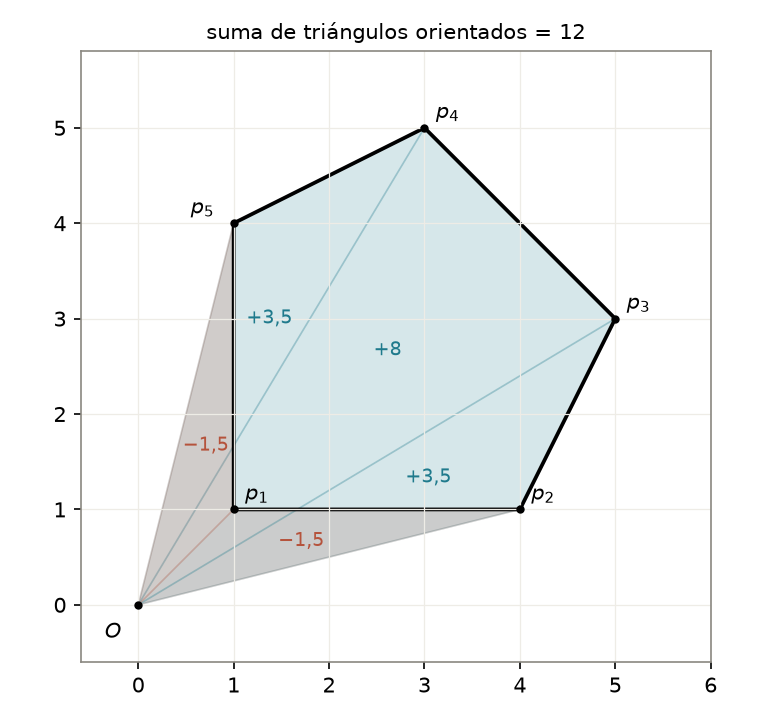
\includegraphics[width=.58\linewidth]{figuras/cuna-determinante/cuna_poligono.png}
\caption{El pentágono \(p_1=(1,1)\), \(p_2=(4,1)\), \(p_3=(5,3)\), \(p_4=(3,5)\),
\(p_5=(1,4)\), descompuesto en los triángulos \(O\,p_i\,p_{i+1}\). Los de \(p_1p_2\) y
\(p_5p_1\) se recorren en sentido horario y aportan \(-1{,}5\) cada uno; los otros aportan
\(3{,}5\), \(8\) y \(3{,}5\). La suma, \(12\), es el área del pentágono. Generada con
\texttt{apunte/scripts/cap06\_cuna\_determinante.py}.}
\label{fig:cuna-poligono}
\end{figure}

\begin{proposicion}[Área de un polígono por cuñas]\label{prop:area-poligono}
Si \(p_1,\dots,p_n\) son los vértices de un polígono simple recorridos en orden y
\(p_{n+1}=p_1\),
\[
  S=\frac12\sum_{i=1}^{n}p_i\wedge p_{i+1}=\frac12\sum_{i=1}^{n}\bigl(x_iy_{i+1}-x_{i+1}y_i\bigr)
\]
es el área del polígono con signo: positiva si el recorrido es antihorario y negativa si es
horario. El valor no cambia si se traslada el origen, ni si se aplica a los vértices una
rotación.
\end{proposicion}

\begin{demostracion}
La descomposición en triángulos desde el origen da la fórmula, como explica la figura: cada
punto interior del polígono queda cubierto una vez más por triángulos positivos que por
negativos, y cada punto exterior, la misma cantidad de veces por unos y por otros. Para la
invariancia ante traslaciones, sea \(c\) un punto cualquiera y \(p_i'=p_i-c\). Por
linealidad y \(c\wedge c=0\),
\[
  \sum_i p_i'\wedge p_{i+1}'=\sum_i p_i\wedge p_{i+1}-\sum_i p_i\wedge c-\sum_i c\wedge p_{i+1}
  =\sum_i p_i\wedge p_{i+1}-s\wedge c-c\wedge s ,
\]
donde \(s=\sum_ip_i\) y usamos que \(\sum_ip_{i+1}=\sum_ip_i\) (es la misma suma, corrida un
lugar). Como \(c\wedge s=-\,s\wedge c\), los dos últimos términos se cancelan. Para una
rotación \(R\),
\(Rp\wedge Rq=\det[Rp\ Rq]=\det\bigl(R\,[p\ q]\bigr)=\det R\,(p\wedge q)=p\wedge q\), por la
proposición~\ref{prop:det-producto} y porque \(\det R=1\).
\end{demostracion}

\begin{idea}[El origen es auxiliar: la superficie no depende de dónde se mida]
Los triángulos desde el origen son un andamio: cambian si se mueve el origen, pero su suma
con signo no. Por eso se puede elegir el origen más cómodo para calcular, por ejemplo uno de
los vértices, y la fórmula del agrimensor da lo mismo en cualquier sistema que difiera del
original por un movimiento rígido.
\end{idea}

\subsection{Aplicación topográfica: superficie de una parcela por coordenadas}\label{sec:aplicacion-superficie}

Una parcela rural se relevó y sus seis vértices quedaron en coordenadas Gauss-Krüger, faja 5,
en metros:

\begin{center}
\small
\begin{tabular}{crrrr}
\toprule
vértice & \(E\) & \(N\) & \(x=E-E_1\) & \(y=N-N_1\)\\
\midrule
\(V_1\) & \(5\,431\,218{,}47\) & \(6\,152\,304{,}12\) & \(0{,}00\) & \(0{,}00\)\\
\(V_2\) & \(5\,431\,507{,}83\) & \(6\,152\,351{,}60\) & \(289{,}36\) & \(47{,}48\)\\
\(V_3\) & \(5\,431\,596{,}25\) & \(6\,152\,158{,}94\) & \(377{,}78\) & \(-145{,}18\)\\
\(V_4\) & \(5\,431\,472{,}10\) & \(6\,151\,987{,}33\) & \(253{,}63\) & \(-316{,}79\)\\
\(V_5\) & \(5\,431\,260{,}66\) & \(6\,151\,962{,}78\) & \(42{,}19\) & \(-341{,}34\)\\
\(V_6\) & \(5\,431\,149{,}39\) & \(6\,152\,121{,}05\) & \(-69{,}08\) & \(-183{,}07\)\\
\bottomrule
\end{tabular}
\end{center}

\paragraph{La fórmula del agrimensor.} Por la proposición~\ref{prop:area-poligono}, la
superficie es \(\tfrac12\bigl|\sum_i(x_iy_{i+1}-x_{i+1}y_i)\bigr|\): la fórmula de Gauss, o
del agrimensor, no es otra cosa que la suma de los cuñas de vértices consecutivos. Las dos
últimas columnas de la tabla son las \emph{coordenadas reducidas}: restamos \(V_1\) a todos
los vértices, lo que la proposición permite sin cambiar el resultado. Con ellas los seis
términos son
\[
  0;\quad -59\,946{,}279;\quad -82\,854{,}923;\quad -73\,208{,}694;\quad -31\,303{,}491;\quad 0
  \quad(\text{m}^2),
\]
(el primero y el último se anulan porque contienen a \(V_1\), que quedó en el origen) y
\[
  S=\tfrac12\,(-247\,313{,}387)=-123\,656{,}693\ \text{m}^2 .
\]

\paragraph{El signo.} \(S\) salió negativa: los vértices están numerados en sentido horario
(\(V_1\) al noroeste, \(V_2\) al noreste, \(V_3\) al este y así siguiendo). Recorridos al
revés, \(V_6,V_5,\dots,V_1\), la suma da \(+123\,656{,}693\) m\(^2\). La superficie es el
valor absoluto,
\[
  \boxed{\ S=123\,656{,}693\ \text{m}^2\approx12{,}366\ \text{ha}\ }
\]
y el signo es un control gratuito del orden de los vértices: si en una planilla aparece un
signo inesperado, algún vértice está fuera de orden.

\paragraph{Por qué reducir las coordenadas.} Con las coordenadas completas cada producto
\(x_iy_{i+1}\) es del orden de \(5{,}4\cdot10^6\times6{,}2\cdot10^6\approx3{,}34\cdot10^{13}\)
m\(^2\), un número de catorce cifras, y la suma final, de seis cifras enteras, es la
diferencia entre números enormes casi iguales. En una calculadora que trabaja con \(12\)
cifras significativas cada producto se redondea a la centena de metros cuadrados, y la fórmula
con coordenadas completas da \(S=-123\,600\) m\(^2\): un error de \(56{,}69\) m\(^2\). Con
las coordenadas reducidas, que tienen a lo sumo cinco cifras, la misma calculadora da
\(-123\,656{,}6933\) m\(^2\), exacto en todas las cifras que muestra. Aun en la doble
precisión de una computadora (unas \(16\) cifras), la fórmula con coordenadas completas da
\(-123\,656{,}691\) m\(^2\), \(0{,}0019\) m\(^2\) lejos del valor correcto: poco, pero
evitable. Reducir al primer vértice es gratis, porque la superficie no depende del origen.

\paragraph{Verificación por triángulos.} Con el origen en \(V_1\), los términos de la fórmula
no nulos son el doble de las áreas con signo de los triángulos en abanico \(V_1V_iV_{i+1}\),
todas negativas por el recorrido horario; en valor absoluto,
\[
  V_1V_2V_3:\ 29\,973{,}140;\quad V_1V_3V_4:\ 41\,427{,}461;\quad
  V_1V_4V_5:\ 36\,604{,}347;\quad V_1V_5V_6:\ 15\,651{,}745\ \ (\text{m}^2),
\]
que suman \(123\,656{,}693\) m\(^2\). Un control independiente de las coordenadas es calcular
cada triángulo con la fórmula de Herón a partir de sus tres lados; por ejemplo,
\(V_1V_2V_3\) tiene lados \(293{,}230\), \(211{,}981\) y \(404{,}716\) m y da otra vez
\(29\,973{,}140\) m\(^2\), y lo mismo los otros tres.

\paragraph{Invariancia ante una rotación.} Si las coordenadas reducidas se giran \(30^\circ\)
con \(R(30^\circ)\), como ocurre al pasar a un sistema local girado respecto de la
cuadrícula, \(V_2\) pasa a \((226{,}853;\ 185{,}799)\), \(V_3\) a \((399{,}757;\ 63{,}160)\), y
así con los demás. Todas las coordenadas cambian, pero \(\det R(30^\circ)=1\) y la fórmula
del agrimensor da otra vez \(-123\,656{,}693\) m\(^2\) (la diferencia, \(1{,}5\cdot10^{-11}\)
m\(^2\), es redondeo de la máquina). Un movimiento rígido no cambia la superficie; una
transformación con \(\det\neq\pm1\), como el paso a un sistema con factor de escala, sí la
cambia, y en la proporción \(|\det|\).

\section{Ejercicios con solución}

\begin{ejercicio}\label{ex:cuna-colineales}
(a) ¿Son colineales \(a=(2,-1)\) y \(b=(-6,3)\)? (b) Calcular el área del paralelogramo de
lados \(u=(2,5)\) y \(v=(4,-1)\) y decir en qué sentido se gira de \(u\) a \(v\).
\end{ejercicio}
\solucion{(a) \(a\wedge b=2\cdot3-(-1)(-6)=6-6=0\): son colineales; en efecto,
\(b=-3a\). (b) \(u\wedge v=2\cdot(-1)-5\cdot4=-22\). El área es \(22\) y el signo negativo
dice que de \(u\) a \(v\) se gira en sentido horario: \(v\) queda a la derecha de \(u\).}

\begin{ejercicio}\label{ex:cuna-rectas}
Hallar con cuñas homogéneas la recta que pasa por \((2,1)\) y \((5,3)\), su punto de corte
con la recta \(x+y=6\) y su ``punto de corte'' con \(2x-3y+4=0\). Interpretar el último
resultado.
\end{ejercicio}
\solucion{\(\ell=(2,1,1)\times(5,3,1)=(1\cdot1-1\cdot3,\ 1\cdot5-2\cdot1,\ 2\cdot3-1\cdot5)
=(-2,3,1)\): la recta \(-2x+3y+1=0\) (control: \(-4+3+1=0\), \(-10+9+1=0\)). Con
\(m=(1,1,-6)\), \(\ell\times m=(-19,-11,-5)\), es decir, el punto \((3{,}8;\ 2{,}2)\);
control: \(3{,}8+2{,}2=6\) y \(-7{,}6+6{,}6+1=0\). Con \((-2,3,4)\), que es la recta
\(2x-3y+4=0\) multiplicada por \(-1\), \(\ell\times(-2,3,4)=(9,6,0)\): tercera coordenada
nula, un punto impropio. Las rectas son paralelas y el resultado es su dirección común,
\((9,6)\sim(3,2)\).}

\begin{ejercicio}\label{ex:cuna-nucleo}
Sea \(A=\begin{pmatrix}1&2&3\\4&5&6\\7&8&9\end{pmatrix}\). Calcular \(\det A\), el núcleo, el
rango y la ecuación implícita de la imagen.
\end{ejercicio}
\solucion{\(\det A=0\) (la tercera fila es el doble de la segunda menos la primera). El cuña
de las dos primeras filas es \((1,2,3)\times(4,5,6)=(2\cdot6-3\cdot5,\ 3\cdot4-1\cdot6,\
1\cdot5-2\cdot4)=(-3,6,-3)\), y \(A(-3,6,-3)^T=0\): el núcleo es la recta de dirección
\((1,-2,1)\). Rango \(3-1=2\). La imagen es el plano generado por las columnas
\((1,4,7)\) y \((2,5,8)\); su normal es el cuña de ellas, \((-3,6,-3)\sim(1,-2,1)\), y la
ecuación es \(x-2y+z=0\), un subespacio lineal de dimensión \(2\). (Que la normal de la
imagen coincida con el núcleo es una casualidad de esta matriz, no una regla.)}

\begin{ejercicio}\label{ex:cuna-plano-afin}
Hallar la ecuación implícita del plano que pasa por \((1,0,0)\), \((0,2,0)\) y \((0,0,3)\).
¿Es un subespacio lineal o afín? Escribir el subespacio lineal paralelo y calcular el volumen
del tetraedro que forma con el origen.
\end{ejercicio}
\solucion{Generadores: \((0,2,0)-(1,0,0)=(-1,2,0)\) y \((0,0,3)-(1,0,0)=(-1,0,3)\). Normal:
\((-1,2,0)\times(-1,0,3)=(6,3,2)\). Como \((6,3,2)\cdot(1,0,0)=6\), el plano es
\(6x+3y+2z=6\): no pasa por el origen, es afín. Su paralelo lineal es \(6x+3y+2z=0\). El
volumen del tetraedro es \(\tfrac16\,\lvert\det[p_1\ p_2\ p_3]\rvert=\tfrac16\cdot6=1\).}

\begin{ejercicio}\label{ex:cuna-cuadrilatero}
Un lote cuadrangular tiene vértices, en metros y en coordenadas locales, \((0,0)\),
\((120,10)\), \((130,95)\) y \((-5,80)\). Calcular su superficie en m\(^2\) y en ha, decir en
qué sentido están numerados los vértices y comprobar que el resultado no cambia si a todas
las coordenadas se les suma \((5\,431\,000;\ 6\,152\,000)\).
\end{ejercicio}
\solucion{Términos \(x_iy_{i+1}-x_{i+1}y_i\): \(0\), \(120\cdot95-130\cdot10=10\,100\),
\(130\cdot80-(-5)\cdot95=10\,875\) y \(0\). \(S=\tfrac12\,(20\,975)=10\,487{,}5\)
m\(^2\)\(\ =1{,}04875\) ha. El signo positivo indica numeración antihoraria. Con las
coordenadas trasladadas la fórmula da otra vez \(10\,487{,}5\) m\(^2\), como asegura la
proposición~\ref{prop:area-poligono}; a mano conviene, sin embargo, trabajar con las
coordenadas chicas.}
